\documentclass[a4paper,10pt,oneside]{article}
\usepackage{latexsym}
\usepackage{amsmath}
\usepackage{amsfonts}
\usepackage{amsthm}
\usepackage{amssymb}
\usepackage{fncylab}
\usepackage{tikz}
\usepackage{url}
\usepackage[bookmarks, colorlinks=false, 
            pdftitle={Úvod do programování --- Algoritmy},
            pdfauthor={Jonathan L. Verner}, 
            pdfsubject={Algoritmy a složitost}, 
            pdfkeywords={algoritmus, složitost, python, třídění, grafy}
            ]{hyperref}
\hypersetup{
    colorlinks,%
    citecolor=black,%
    filecolor=black,%
    linkcolor=black,%
    urlcolor=black
}
\usepackage[margin=1cm]{geometry}
\usetikzlibrary{decorations.fractals}
\usepackage[utf8]{inputenc}
\relpenalty=9999
\binoppenalty=9999


%----------definitions---------------------------


%math definitions

\newcommand{\R}{\mathbb R}
\newcommand{\C}{{\mathcal C}}
\newcommand{\F}{{{\mathcal F}}}
\newcommand{\U}{{{\mathcal U}}}
\newcommand{\V}{{{\mathcal V}}}
\newcommand{\cont}{{\mathfrak{c}}}
\newcommand{\force}{\Vdash}
\newcommand{\pw}{{{\mathcal P}}}
\newcommand{\MU}{{\mathbb{M}_{\mathcal{U}}}}
\newcommand{\pomega}{\pw(\omega)}






%---------numbering of the theorems------------
 \swapnumbers

 \newtheorem*{theorem*}{Theorem}
 \newtheorem{theorem}[subsection]{Theorem}
 \newtheorem{proposition}[subsection]{Proposition}
 \newtheorem{observation}[subsection]{Pozorování}
 \newtheorem*{observation*}{Pozorování}
 \newtheorem{fact}[subsection]{Fact}
 \newtheorem{lemma}[subsection]{Lemma}
 \theoremstyle{definition}
 \newtheorem{definition}[subsection]{Definice}
 \newtheorem{question}[subsection]{Problém}
 \newtheorem{ukol}[subsection]{Úloha}
 \newtheorem{cviceni}[subsection]{Cvičení}
 \newtheorem*{comments*}{Komentáře}
 \newtheorem*{definition*}{Definice}
 \newtheorem*{question*}{Question}
 \newtheorem{notation}[subsection]{Notation}
 \newtheorem{remark}[subsection]{Remark}
 \newtheorem*{note}{Pozn}
 \newtheorem*{ack}{Acknowledgements}
 
% \pdfinfo{
%      /Author ()
%      /Title ()
%      /Subject (2010 MSC: Primary )
%      /Keywords ()
%   }
\include{pythonlisting}
\lstset{
numbers=left,
stepnumber=1,
numbersep=0pt,
numberstyle=\small\color{black}
}
%-------------opening--------------------------
\begin{document}
\title{}

% \author{Jonathan Verner}
% \address{Department of Logic, Charles University\\
% Palachovo nám. 2\\ 116 38 Praha 1, Czech Republic}
% \email{jonathan.verner{@}ff.cuni.cz}
%\thanks{The author was partially supported by }

%\subjclass[2010]{Primary }
%\keywords{}

%\begin{abstract}
%\end{abstract}
%\maketitle
\thispagestyle{empty}
\pagestyle{empty}
%\hsize=16cm
\parindent=0cm
\parskip=0.2cm

\begin{center}
\section*{Grafové algoritmy II}
\end{center}
\addtocounter{section}{1}

\subsection{Nejkratší cesta}


\begin{definition} \emph{Erdösovo číslo} je definováno následovně. Erdös má Erdösovo číslo 0. Každý člověk, který publikoval článek s Erdösem
má číslo jedna. Každý člověk, který publikoval článek s člověkem s Erdösovým číslem 1 má číslo 2... Tedy Erdösovo číslo $e$ člověka $p$
je definováno:
\begin{displaymath}
 e(p) = 
 \begin{cases}
 0\quad\mbox{je-li $p$ Erdös}\\
 \min\{ e(c)+1:\mbox{$p$ a $c$ publikovali společný článek}\}\cup\{\infty\}\quad\mbox{jinak}
 \end{cases}
\end{displaymath}
\end{definition}


\begin{question} Napište program, který počítá Erdösova čísla.
\end{question}


Pro výpočet budeme mít zadán následující graf: vrcholy v grafu budou odpovídat jednotlivým lidem, hrany mezi dvěmi vrcholy budou odpovídat
společnému článku. Úlohu vyřešíme jednoduchým procházením do šířky. V proměnné {\tt prace} si budeme uchovávat vrcholy, které je ještě třeba
navštívit a ke každému vrcholu i horní odhad jeho Erdösova čísla. V proměnné {\tt ret} si ke každému vrcholu budeme pamatovat nejmenší horní
mez Erdösova čísla, na kterou jsme dosud při procházení narazili. Pokaždé, když navštívíme vrchol podíváme se, zda je potřeba upravit
proměnnou ret (t.j. buď jsme ve vrcholu poprvé, pak si v proměnné ret si uložíme aktuální horní odhad jeho čísla, nebo jsme zde již byli, 
ale aktuální horní odhad je menší než máme v {\tt ret} uložený a musíme ho tedy upravit). Pokud jsme proměnnou {\tt ret} musíme ještě někdy v budoucnosti
navštívit sousedy aktuálního vrcholu s novým odhadem, proto je přidáme do proměnné {\tt prace}. V okamžiku, kdy bude proměnná {\tt prace} prázdná,
bude mít každý vrchol grafu, do kterého vede z $e$ cesta přiřazeno v proměnné {\tt ret} své definitivní Erdösovo číslo. Ostatní vrcholy nemají 
Erdösovo číslo rozumně definované, resp. mají je $\infty$.

V pythonu může program vypadat třeba následovně:

\begin{python}
 from collections import deque
 def erdos( e, graf ):
    prace = deque( [ (0, e) ] )
    ret = {}
    while( len(prace) > 0 ):
        (e_num,v) = prace.popleft()
        if ( v in ret and ret[v] > e_num ) or ( v not in ret):
            ret[v] = e_num
            for s in graf[v]:
                prace.append( e_num+1, s )
    return ret
\end{python}


\begin{note} Výše uvedený kód používá typ {\tt deque}, se kterým jsme se dosud nesetkali. Typ deque se chová jako fronta (t.j. first in first out, FIFO,
prvky se přidávají nakonec, odebírají se ze začátku). U obyčejného {\tt list}u lze odebírat prvky ze začátku, ale tato operace je velmi pomalá
(celé pole se následně musí přesunout). Typ {\tt deque} je implementován tak, aby operace odebírání ze začátku měla konstantní složitost. 
\end{note}

Ještě se přesvědčíme, že se program opravdu funguje. Nejprve ukážeme, že se nezacyklí, t.j. že skončí. Všimněme, že Erdösovo číslo každého vrcholu je 
shora omezené počtem všech vrcholů $n$, tedy v proměnné {\tt ret} bude pro daný vrchol v nejhorším případě uložené číslo $n$. Dále, kdykoliv ve vrcholu něco 
děláme, musíme snížit proměnnou {\tt ret}. Po nejvýše $n^2$ krocích se tedy musíme dostat do situace, kdy už v žádném vrcholu nic dělat nebudeme, 
Pak už jen vyprázdníme proměnnou {\tt prace} a program skončí. Tedy program se nemůže zacyklit. 

Nyní ukážeme, že opravdu počítá Erdösova čísla správně. Ukážeme si to tzv. sporem --- budeme předpokládat, že program počítá čísla špatně a zjistíme, že to není
možné. Předně je jasné, že pokud se zmýlí, tak se zmýlí směrem nahoru --- tzn. vrátí Erdösovo číslo větší, než má ve skutečnosti být. Předpokládejme, že
se program zmýlil a zvolme si vrchol $v$ tak, aby {\tt ret[$v$]} bylo mezi špatně spočtenými čísly nejmenší. Nyní vrchol $v$ musí mít nějakého souseda $s$,
který má Erdösovo číslo rovné {\tt ret[$v$]-1}. Toto číslo ale musí být správné, protože vrchol je $v$ nejmenší špatný. Z definice Erdösova čísla nyní plyne,
že $e(v)\leq${\tt ref[$v$]}, tedy hodnota $v$ byla ve skutečnosti správná, což není možné.

Pojdmě se nyní zamyslet co by se stalo, kdybychom řádek šest nahradili řádkem:

\begin{python}
        v = prace.pop()
\end{python}

Program by opět procházel grafem a počítal Erdösova čísla, nicméně pořadí procházení by bylo jiné. Šlo by o tzv. procházení do hloubky (pamatujte:
fronta = procházení do šířky, zásobník = procházení do hloubky). 

\begin{center}
\begin{minipage}{9cm}
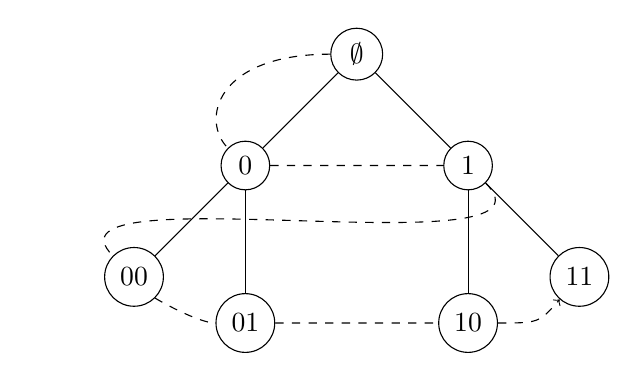
\begin{tikzpicture}[node distance=2cm]
\tikzstyle{vertex}=[draw,circle]
\node [vertex] (empty){$\emptyset$};
\node [vertex,below left of = empty] (0) {0};
\node [vertex,below right of = empty] (1) {1};
\node [vertex,below left of = 0] (00) {00};
\node [vertex,below of = 0] (01) {01};
\node [vertex,below of = 1] (10) {10};
\node [vertex,below right of = 1] (11) {11};
\path[every node/.style={font=\sffamily\small}]
    (empty) edge node {} (0)
    (empty) edge node {} (1)
    (0) edge node {} (00)
    (0) edge node {} (01)
    (1) edge node {} (10)
    (1) edge node {} (11);
\draw[dashed,->]
    (empty)..controls +(west:1.8) and +(north west:0.8) ..(0) 
           ..controls +(east:0.8) ..(1) 
           ..controls +(south east:1.9) and +(north west:1.9) ..(00)
           ..controls +(south east:0.4) and +(west:0.6)..(01)
           ..controls +(east:0.9) ..(10)
           ..controls +(east:0.9) ..(11);
\end{tikzpicture}
\end{minipage}
\begin{minipage}{9cm}
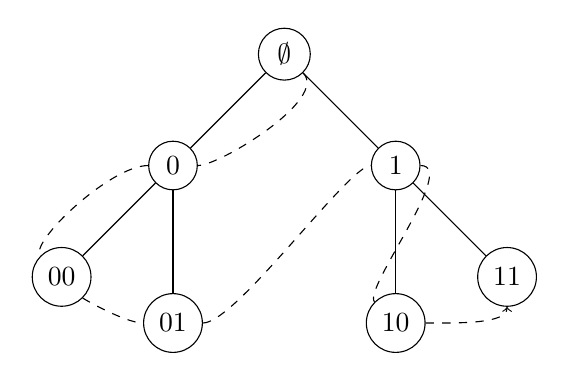
\begin{tikzpicture}[node distance=2cm]
\tikzstyle{vertex}=[draw,circle]
\node [vertex] (empty){$\emptyset$};
\node [vertex,below left of = empty] (0) {0};
\node [vertex,below right of = empty] (1) {1};
\node [vertex,below left of = 0] (00) {00};
\node [vertex,below of = 0] (01) {01};
\node [vertex,below of = 1] (10) {10};
\node [vertex,below right of = 1] (11) {11};
\path[every node/.style={font=\sffamily\small}]
    (empty) edge node {} (0)
    (empty) edge node {} (1)
    (0) edge node {} (00)
    (0) edge node {} (01)
    (1) edge node {} (10)
    (1) edge node {} (11);
\draw[dashed,->]
    (empty)..controls +(south east:0.8) and +(east:0.6) ..(0) 
           ..controls +(west:0.8) and +(north west:0.6) ..(00)
           ..controls +(south east:0.4) and +(west:0.6) ..(01)
           ..controls +(east:0.8) and +(west:0.6) ..(1)
           ..controls +(east:0.8) and +(north west:0.6) ..(10)
           ..controls +(east:0.8) and +(south:0.6) ..(11);
\end{tikzpicture}
\end{minipage}

\vskip1cm
{\it Procházení do hloubky vs. do šířky}
\end{center}


Pro některé grafy nebude mít tato změna vliv žádný. 

\begin{cviceni} Nalezněte graf, pro který procházení do šířky splývá s procházením do hloubky.
\end{cviceni}

Nicméně pro většinu reálných grafů to bude mít vliv podstatný. Při vyhledávání do šířky totiž každý vrchol navštívíme maximálně jednou. V okamžiku,
kdy ho navštívíme, známe jeho Erdösovo číslo --- daný vrchol nemůže mít Erdösovo číslo menší, protože pak by se nacházel na nižší hladině, tudíž
bychom ho při procházení do šířky již navštívili. Pokud však budeme prohledávat do hloubky, typicky navštívíme každý vrchol mnohokrát. Navíc, vzhledem
k tomu, že většina lidí má Erdösovo číslo menší než 5 (tento fakt souvisí s tzv. \emph{small world penomenon}, viz například 
\url{http://en.wikipedia.org/wiki/Small_world_phenomenon}) to bude pro většinu vrcholů naprosto zbytečná práce

Výhoda procházení do šířky při počítání Erdösova čísla tedy spočívá v tom, že vrcholy ve skutečnosti procházíme v pořadí podle jejich Erdösových čísel.
Vyslovme to jako pozorování:

\begin{observation*} Je-li $e(v_1) < e(v_2)$ pak při procházení do šířky navštívíme vrchol $v_1$ dříve než navštívíme vrchol $v_2$.
\end{observation*}

Díky tomuto pozorování můžeme náš výše uvedený algoritmus dokonce ještě trochu vylepšit. Na řádku 7 totiž nemusíme testovat, zda je hodnota uložená
v {\tt ret} vyšší, než hodnota, kterou bychom tam chtěli vložit. Pokud tam totiž nějaká už hodnota je, tedy jsme daný vrchol již navštívili, je ta
hodnota jistě menší. Řádek 7 tedy lze nahradit řádkem:
\begin{python}
            if v not in ret: 
\end{python}
Zkusme nyní ještě program upravit tak, aby kromě Erdösových čísel počítal i cesty, které tato čísla dosvědčují --- t.j. ke každému vrcholu $v$ nalezne
cestu z $e$ do $v$ délky $e(v)$. K tomu stačí malá úprava: v u každého vrcholu si budeme kromě jeho čísla pamatovat také jeho souseda, který má číslo
o jedna menší. Najít cestu z $e$ do $v$ (resp. z $v$ do $e$) pak bude jednoduché. Začneme ve vrcholu $e$, přejdeme k sousedovi s o jedna menším číslem 
a tak budeme postupovat dokud se nedostaneme do $e$. Program může vypadat například následovně. 
\begin{python}
 from collections import deque
 def varerdos( e, graf ):
    prace = deque( [ (0,e,e) ] )
    cisla = {}
    while( len(prace) > 0 ):
        (num, prev, cur) = prace.popleft()
        if cur not in cisla:
            cisla[cur]=(prev,num)
            for s in graf[cur]:
                prace.append( (num+1,cur,s) )
    return cisla
 
 def cesta(e, v, cisla):
    ret = []
    if v not in cisla:
        return None
    while( not v == e ):
        ret.append(v)
        v = cisla[v][0]
    return ret
\end{python}

Jistě jste si všimli, že Erdösovo číslo ve skutečnosti odpovídá vzdálenosti vrcholu $v$ od vrcholu $e$. Předcházející program tak vlastně našel
nejkratší cesty z vrcholu $e$ do všech ostatních vrcholů. Podíváme se teď na variantu této úlohy. Co kdybychom nechtěli nejkratší cestu co se počtu
hran týče, ale nejkratší z nějakého jiného hlediska. Každá hrana může mít například přiřazenou nějakou délku a pak by nám šlo o nejkratší cestu
vzhledem k těmto délkám:

\begin{question} Je dán graf a ke každé hraně v grafu je navíc zadáno kladné číslo. Nalezněte cestu z vrcholu a do vrcholu b tak, 
aby součet těchto čísel na dané cestě byl co nejmenší.
\end{question}

Tato úloha je velmi podobná té předchozí s jedným podstatným rozdílem. I pokud budeme procházet grafem do šířky, nebudeme už mít zaručeno, že
v okamžiku, kdy nějaký vrchol navštívíme poprvé, dostaneme se tam nejkratší cestou. To je pěkně vidět na následujícím obrázku (přerušovaná čára
ukazuje v jakém pořadí se prochází vrcholy při procházení do šířky):


\begin{center}
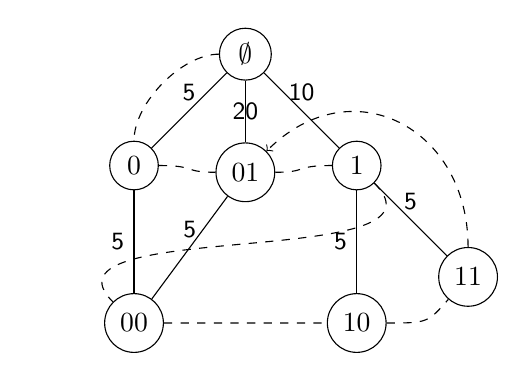
\begin{tikzpicture}[node distance=2cm]
\tikzstyle{vertex}=[draw,circle]
\node [vertex] (empty){$\emptyset$};
\node [vertex,below left of = empty] (0) {0};
\node [vertex,below right of = empty] (1) {1};
\node [vertex,below of = 0] (00) {00};
\node [vertex,below of = empty] at (0,0.5) (01) {01};
\node [vertex,below of = 1] (10) {10};
\node [vertex,below right of = 1] (11) {11};
\path[every node/.style={font=\sffamily\small}]
    (empty) edge node [above] {5} (0)
    (empty) edge node [above] {10} (1)
    (empty) edge node {20} (01)
    (0) edge node [left] {5} (00)
    (00) edge node [above] {5} (01)
    (1) edge node [left] {5} (10)
    (1) edge node [above] {5} (11);
\draw[dashed,->]
    (empty)..controls +(west:0.8) and +(north:0.8) ..(0)
           ..controls +(east:0.8) and +(west:0.8) ..(01)
           ..controls +(east:0.8) and +(west:0.8)..(1) 
           ..controls +(south east:1.9) and +(north west:1.9) ..(00)
           ..controls +(east:0.8) and +(west:0.8)..(10)
           ..controls +(east:0.9) ..(11)
           ..controls +(north:1.9) and +(north east:1.9) ..(01);
\end{tikzpicture}
\end{center}

Zde je vidět, že při první návštěvě vrcholu $01$ jsme se tam dostali cestou délky 20, zatímco při druhé návštěve (poslední navštívený
vrchol), jsme se tam dostali cestou délky 15. Abychom dostali funkční program, musíme se vrátit k původní verzi sedmého řádku. Tak získáme
funkční program, nicméně nebude příliš efektivní.

Dijsktrův algoritmus, který si nyní ukážeme, je založený na modifikované myšlence procházení do šířky. Nakresleme si ještě jednou předcházející
situaci tak, že si vrcholy uspořádáme do hladin podle vzdálenosti od vrcholu $\emptyset$. Kdyby se nám podařilo procházet tímto grafem po hladinách 
(t.j. ``do šířky'') tak, jak je to na obrázku nakresleno, měli bychom zaručeno, že v okamžiku kdy vrchol navštívíme, dostali jsme se tam nejkratší
možnou cestou:

\begin{center}
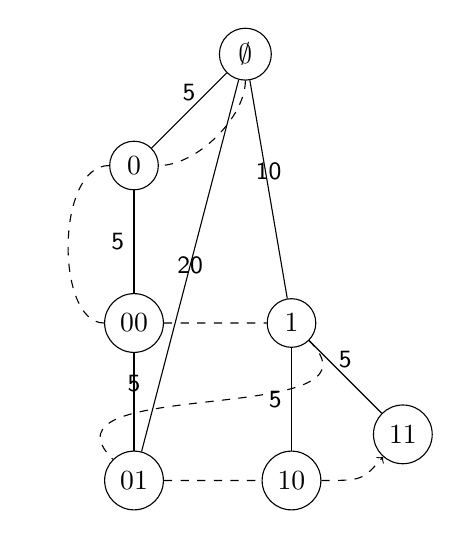
\begin{tikzpicture}[node distance=2cm]
\tikzstyle{vertex}=[draw,circle]
\node [vertex] (empty){$\emptyset$};
\node [vertex,below left of = empty] (0) {0};
\node [vertex,below of = 0] (00) {00};
\node [vertex,right of = 00] (1) {1};
\node [vertex,below of = 00] (01) {01};
\node [vertex,below of = 1] (10) {10};
\node [vertex,below right of = 1] (11) {11};
\path[every node/.style={font=\sffamily\small}]
    (empty) edge node [above] {5} (0)
    (empty) edge node [above] {10} (1)
    (empty) edge node {20} (01)
    (0) edge node [left] {5} (00)
    (00) edge node [above] {5} (01)
    (1) edge node [left] {5} (10)
    (1) edge node [above] {5} (11);
\draw[dashed,->]
    (empty)..controls +(south:0.8) and +(east:0.8) ..(0)
           ..controls +(west:1) and +(west:1) ..(00)
           ..controls +(east:0.8) and +(west:0.8)..(1) 
           ..controls +(south east:1.9) and +(north west:1.9) ..(01)
           ..controls +(east:0.8) and +(west:0.8)..(10)
           ..controls +(east:0.9) ..(11);
\end{tikzpicture}
\end{center}

Dijkstrův algoritmus toho docílí tak, že si v každém kroku pamatuje, který z dosud nenavštívených vrcholů se nachází nejblíže počátečnímu vrcholu
a ten navštíví v následujícím kroku. Implementace v pythonu je téměř totožná s druhou verzí našeho programu, stačí s proměnnou {\tt prace} pracovat
jako s haldou. K tomu nám poslouží Pythonovská knihovna {\tt heapq} a její funkce {\tt heappop} a {\tt heappush}. Pro úplnost uvedeme plný kód:

\begin{python}
 import heapq
 def dijkstra( e, graf ):
    prace = [ (0,e,e) ]
    cisla = {}
    while( len(prace) > 0 ):
        (num, prev, cur) = heapq.heappop(prace)
        if cur not in cisla:
            cisla[cur]=(prev,num)
            for s in graf[cur]:
                heapq.heappush( prace, (num+1,cur,s) )
    return cisla
\end{python}



% \bibliographystyle{mujstyl}
% \bibliography{ref}

\end{document}


